\documentclass[conference]{IEEEtran}
\hyphenation{op-tical net-works semi-conduc-tor}

\usepackage{float}
\usepackage{graphicx}
\usepackage{hyperref}

\begin{document}
\title{A Database Management System for a Geospatially-Enabled Interactive Game}
\author{\IEEEauthorblockN{Arturo Casillas}
\IEEEauthorblockA{\small Southern Methodist University\\
Dallas, Texas\\
Email: acasillas@smu.edu}
\and
\IEEEauthorblockN{Rene Pineda}
\IEEEauthorblockA{\small Southern Methodist University\\
Dallas, Texas\\
Email: rpinedaalvarenga@smu.edu}
\and
\IEEEauthorblockN{Volodymyr Orlov}
\IEEEauthorblockA{\small Southern Methodist University\\
Dallas, Texas\\
Email: vorlov@smu.edu}
\and
\IEEEauthorblockN{Vitaly Briker}
\IEEEauthorblockA{\small Southern Methodist University\\
Dallas, Texas\\
Email: vbriker@gmail.com}}

\maketitle

\begin{abstract}
The success of Pokémon Go\footnote[1]{Pokémon Go Wikipedia page: https://goo.gl/LeX1D3} and its predecessor, Ingress\footnote[2]{Ingress Wikipedia page: https://goo.gl/6VXFoC} demonstrates that the users of smartphones respond positively and engage with interactive technologies such as augmented reality and location services. Massive online games where players actively move around the world might impose significant technical challenges for a game designer. These issues and possible solutions have note been given enough attention in the literature. This work is based on our experience of design and implementation of geospatially-enabled interactive game and gives an overview of the available database technologies which can be used for multiplayer mobile game where device's GPS coordinates are used to locate and capture virtual tokens. 
\end{abstract}

\IEEEpeerreviewmaketitle

\section{Introduction}
Location based apps and services are becoming more popular and more popular. The game Pokémon Go, in particular, has gained over 44 million users and additionally incorporates augmented reality. We plan to develop a database that can collect, store and aid in processing information for a game where players will be collecting items in different tourist destinations to earn points. The game will consist of players moving around the real world and collecting tokens that gradually reveal parts of a story. The data will be collected from a user interface operating on their cellphones. The emphasis is to design a system that can efficiently collect and store geospatially enabled data, and use a database structure to manage the game rules and possible interactions among players. 

\section{Game rules and design considerations}
\subsection{Problem statement}
As mentioned, the game will consist of players exploring the real world in search of tokens. Collecting tokens raises the player’s score which will in turn reveal a segment of a story once the player’s score reaches a certain threshold. The tokens belong to different categories that correspond to different aspects of the story that may be revealed. As such, this game relies heavily on the search-and-find mechanic as well as desires for collection, completion, and closure of narrative for player engagement \cite{game-methodology, location-based-games}. 
The story is a science fiction story that places the player in the role of an explorer. The player finds himself exploring ruins on another world that once housed an advanced civilization. The player must then find tokens that will divulge information about this lost civilization including clues as to what caused the civilization to disappear. Categories consist of Culture, Politics, Technology, and Economy and correspond to the nature of the clues the player discovers. 
Given the rules, mechanics, and the location-based nature of the game, some data and database design considerations are:

\begin{enumerate}
	\item Nature of GPS Data. Learning GPS data types, how they are stored, and how they may be obtained both from the player and by the player.
	\item Available DBMS. What DMBS and existing software packages work well with GPS data and are also capable of implementing game rules.
	\item Computations GPS Data. What computations can be done with GPS data to enforce game rules and accomplish game mechanics such as the player interacting with geospatial objects.
	\item Database Schema. What entities and attributes are necessary to store and what portions of the game may be saved by the player.
\end{enumerate}
	
\subsection{Previous work related to the problem}
An interesting paper by Chulmo Koo and others investigate relationship between geospatially enabled mobile game and destination satisfaction \cite{destination-engagement}. Besides, some authors argue that location-based games are positively associated with a set of beneficial health behaviors \cite{pokemon-motivation}. We found it interesting that a game can have a positive effect on tourism and person’s wellness and would like to extend research in this area.  
   Initial research in this area brought us to a paper summarizing design patterns possible with location-based games \cite{location-based-mg}. Due to time and resource limits imposed on us we decided to use on Search-and-Find pattern for our game. On the other hand, the large-scale nature of multiplayer games might generate enormous data sets. Effective handling of this data requires a sophisticated database management system \cite{data-store-issues, location-based-services}. In his thesis, Kristian Midtgård looks at the NoSQL landscape in an attempt to find the best practices and candidate databases for achieving high write throughput \cite{massive-amounts-location-data}. We plan to build on top of his research and look at other, more modern databases. 
	
\section{High-level description of the system}
In order to be able to serve big number of requests in a timely manner and scale well with increasing number of players we need a system that will not only have a well designed, scalable database, but also other components integrated into a single, well thought architecture. Our system is built from 3 major components:

\begin{itemize}
  \item Client-side application. We decided to support 2 major platforms that got widespread adoption: Android and iOS. For the proof-of-concept we focused on iOS. 
  \item Backend services, or middle layer. This component performs server-side operations, enforces gameplay rules and handles requests to our database. 
  \item Geospatially enabled database. Here all information regarding our players, tokens and corresponding states is being kept. 
\end{itemize}

We use following communication protocols between these components:

\begin{itemize}
\item REST over HTTP. 
\item SQL 
\end{itemize}

On the client side we use Apple’s Core Location Framework to collect longitude and latitude of a player and Apple’s ARKit to place tokens around player. We calculate bearing and distance between player and a token to place tokens around given user. To uniquely identify each player we use Vendor ID.
We want our backend to support large number of requests coming from multiple players. To achieve that we use multiple copies of the identical services capable to scale up or down depending on the level of load. Luckily we do not have to think about scalability properties of our hardware since we run our services in AWS Cloud on EC2 virtual instances.  To spread load across multiple copies of the backend service we use AWS load balancer that distributes client’s requests in a round-robin fashion between EC2 instances. 
We use AWS to host our database. 
Layout of all three components are represented schematically in \autoref{schema}. 

\begin{figure}
\centering
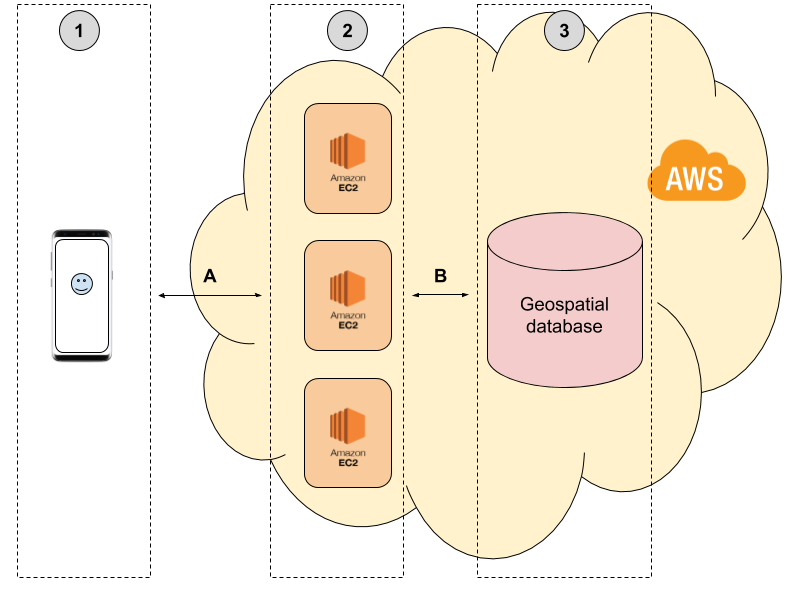
\includegraphics[width=2.5in]{imgs/systemschema.png}
\caption{Schematic layout of major components of the system}
\label{schema}
\end{figure}

\section{Database design}
TBD
\section{Conclusion}
TBD

\section*{Acknowledgment}


The authors would like to thank...


\begin{thebibliography}{1}

\bibitem{game-methodology}
R. Dillon, "The 6-11 Framework: A new methodology for game analysis and design" presented at the Proceedings Game-On Asia Conference, Singapore, Mar., 2011.

\bibitem{location-based-games}
L. Lehman, "Location-based Mobile Games" Technical University of Berlin, unpublished, 2012.
  
\bibitem{destination-engagement}
Koo Chulmo, Choi Kyuwon, Ham Juyeon, Chung Namho. Empirical Study About the PokémonGo Game and Destination Engagement, 2018

\bibitem{pokemon-motivation}
Marquet O, Alberico C, Adlakha D, Hipp JA. Examining motivations to play Pokemon Go and their influence on perceived
outcomes and physical activity. JMIR Serious Games 2017

\bibitem{location-based-mg}
L. Lehmann, Location-Based Mobile Games. GRIN Verlag Munich Germany, 2012.

\bibitem{data-store-issues}
J. Krumm and S. A. Shafer. Data store issues for location-based services. IEEE Data Eng. Bull., 2005.

\bibitem{location-based-services}
Jensen, C., Christensen, A., Pedersen, T., Pfoser, D.,Saltenis, S. and Tryfona, N. (2001). "Location-Based Services: A Database Perspective" Proceedings of Scandinavian GIS

\bibitem{massive-amounts-location-data}
K. Midtgård. Collecting massive amounts of location data in a NoSQL database. Master of Science in Computer Science, Norwegian University of Science and Technology, 2017

\end{thebibliography}

\end{document}


